%! Author = aybehrouz


\section{Introduction}\label{sec:introduction}

The Argennon\footnote{The classical pronunciation should be used:\textipa{/Ar"gen.non/}} Smart Contract Execution
Environment (AscEE) is an abstract execution environment for executing Argennon smarts contracts (a.k.a\ Argennon
applications). An Argennon application essentially is an HTTP server whose state is kept in the Argennon blockchain and
its logic is described using an Argennon Standard Representation (ASR).

An Argennon Standard Representation (ASR) is a programming language for describing argennon applications, optimized
for the architecture and requirements of the Argennon platform.
Argennon supports two standard representations: one is a high level text based language which needs
costly compilation before being executed on a hardware machine. The other is a low level binary representation which
usually can be executed, with minimal pre-processing, by a JIT compiler or an emulator. The high level
language is intended for preserving the high level information of applications logic to facilitate
platform specific compiler optimization at host nodes. The low level language, on the oder hand, is designed for
efficient direct execution of applications that are not frequently used.

The state of an Argennon application is stored in byte addressable finite arrays of memory called
\emph{heap chunks}. An application may have several heap chunks with different sizes, and can remove or
resize its heap chunks or allocate new chunks. Every chunk belongs to exactly one application and can only be modified
by its owner. In addition to heap chunks, every application has an amount of non-persistent local memory for
storing temporary data.

The AscEE executes the requests contained in each block of the Argennon
blockchain in a three-step procedure. The first step is the \emph{preprocessing step}. In this step, the required
data for executing requests are retrieved from the Argennon cloud and the helper data structures are constructed.
This step is
designed in a way that can be done fully in parallel for each request without any risks of data races. The second
step is the \emph{Data Dependency Analysis (DDA) step}.
In this step by analyzing data dependency between requests, the AscEE determines requests that can be run in parallel
and requests that need to be run sequentially. This information is represented using an \emph{execution dag} data
structure and in the final step, requests are executed using that data structure.


\section{Execution Sessions}\label{sec:sessions}

The Argennon Smart Contract Execution Environment can be seen as a machine for executing Argennon applications to
fulfill HTTP requests, produce their HTTP responses and update related heap chunks. The execution of requests can be
considered sequential\footnote{Actually requests are executed in parallel but by performing data dependency analysis the
result is guaranteed to be identical
with sequential execution of requests.} and each request has a separate \emph{execution session}. An execution session
is a separate session of executing smart contract's code in order to fulfill an \emph{external} HTTP request.
External requests are requests that are not made by other Argennon applications.

The state of an execution session will be
destroyed at the end of the session and only the state of heap chunks is preserved. If a session fails and does not
complete normally, it will not have any effect on any heap chunks.

During an execution session an application can make \emph{internal} HTTP requests to other applications. Those
requests will not start a new execution session and will be executed within the current session. In AscEE making an
HTTP request to an application is similar to a function invocation, and for that reason, we also refer to them as
application calls.

The AscEE is designed based on \emph{optional decoupling principle}. When an application makes a request to another
application, optionally it can choose to be decoupled from the called application. That would mean the called
application could not affect its caller's state by reentrancy, or could not fail the session by using excessive
resources or performing illegal operations.


\section{Identifiers}\label{sec:identifiers}

In Argennon a unique identifier is assigned to every application, heap chunk and account. Consequently, three distinct
identifier types exist: \texttt{appID}, \texttt{accountID}, and \texttt{chunkID}.
All these identifiers are \emph{prefix codes}, and hence can be represented by
\emph{prefix trees}\footnote{Also called tries.}.

Argennon has four primitive prefix trees:
\emph{applications, accounts, local} and \emph{varUint}.
All these trees are in base 256, with the maximum height
of 8.

An Argennon identifier may be simple or compound. A simple identifier is generated using a single trie, while a
compound identifier is generated by concatenating prefix codes generated by two or more tries:

\begin{itemize}
    \item \texttt{appID} is a prefix code built by \emph{applications} prefix tree. An \texttt{appID} cannot
    be \texttt{0x0}.

    \item \texttt{accountID} is a prefix code built by \emph{accounts} prefix tree. An \texttt{accountID} cannot
    be \texttt{0x0} or \texttt{0x1}.

    \item \texttt{chunkID} is a composite prefix code built by concatenating an \texttt{applicationID} to
    an \texttt{accountID} to a prefix code made by \emph{local} prefix tree:
    \subitem \texttt{chunkID = (applicationID|accountID|<local-prefix-code>)} .
\end{itemize}

All Argennon prefix trees have an equal branching factor \(\beta\). Therefore, we can represent an Argennon
prefix tree as a sequence of fractional numbers\footnote{It's possible to have \(a_i=0\).
For example, \(A^{(4)}=(0.2000)_{10}\) is correct.} in base \(\beta\):
\[
    (A^{(1)},A^{(2)},A^{(3)},\dots)\ ,
\]
where \(A^{(i)}=(0.a_{1}a_{2}\dots a_{i})_\beta\), and we have \(A^{(i)} \leq A^{(i+1)}\).\footnote{A typical choice for
    \(\beta\) is \(2^8\).}

One important property of prefix identifiers is that while they have variable and unlimited length, they are
uniquely extractable from any sequence. Assume that we have a string of digits in base $\beta$, we
know that the sequence starts with an Argennon identifier, but we do not know the length of that identifier.
Algorithm~\ref{alg:prefix_id} can be used to extract the prefixed identifier uniquely. Also, we can apply this algorithm
multiple times to extract a composite identifier, for example \texttt{chunkID}, from a sequence.

%##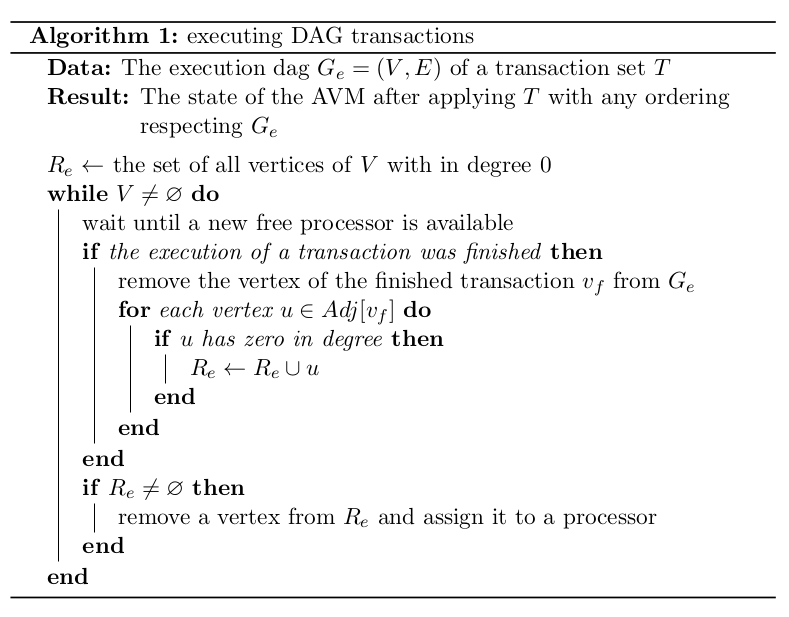
\includegraphics[width=17cm]{../img/Alg1s.png}
\begin{algorithm}[t]
    \DontPrintSemicolon
    \SetKwInOut{Input}{input}\SetKwInOut{Output}{output}
    \Input{A sequence of $n$ digits in base $\beta$: $d_{1}d_{2}\dots d_{n}$ \newline
    A prefix tree: $<A^{(1)},A^{(2)},A^{(3)},\dots>$}
    \BlankLine
    \Output{Valid identifier prefix of the sequence.}
    \BlankLine
    \For{$i = 1$ \KwTo $n$}
    {
        \If{$(0.d_{1}d_{2}\dots d_{i})_\beta < A^{(i)}$}
        {
            \KwRet{$d_{1}d_{2}\dots d_{i}$}\;
        }
    }
    \KwRet{NIL}\;
    \caption{Finding a prefixed identifier}\label{alg:prefix_id}
\end{algorithm}

When we have a prefixed identifier, and we want to know if a sequence of digits is marked by that identifier,
we use Algorithm~\ref{alg:match_id} to match the prefixed identifier with the start of the sequence. The matching
can be done with only three comparisons, and an invalid prefixed identifier can be detected and will not match
any sequence.

In Argennon the shorter prefix codes are assigned to more active accounts and applications which tend to own more
data objects in the system. The prefix trees are designed by analyzing empirical data to make sure the number
of leaves in each level is chosen appropriately.

\begin{algorithm}[h]
    \DontPrintSemicolon
    \SetKwData{Id}{$id$}
    \SetKwInOut{Input}{input}\SetKwInOut{Output}{output}
    \Input{A prefixed identifier in base $\beta$ with $n$ digits: $\Id=a_{1}a_{2}\dots a_{n}$ \newline
    A sequence of digits in base $\beta$: $d_{1}d_{2}d_{3}\dots $ \newline
    A prefix tree: $<0,A^{(1)},A^{(2)},A^{(3)},\dots>$
    }
    \BlankLine
    \Output{$TURE$ if and only if the identifier is valid and the sequence starts with the identifier.}
    \BlankLine
    \If{$(0.a_{1}\dots a_{n})_\beta = (0.d_{1}\dots d_{n})_\beta$}
    {
        \If{$A^{(n-1)} \leq (0.a_{1}a_{2}\dots a_{n})_\beta < A^{(n)}$}
        {
            \KwRet{TRUE}\;
        }
    }
    \KwRet{FALSE}\;
    \caption{Matching a prefixed identifier}\label{alg:match_id}
\end{algorithm}


\section{Heap Chunks}\label{heap}

The persistent data of an Argennon application is stored in heap chunks. An application may have several heap chunks
with different sizes, and can remove or
resize its chunks or allocate new chunks. Every chunk belongs to exactly one application. Only the owner application can
modify a chunk but there is no restrictions for reading a chunk\footnote{The reason behind this type of access
control design is the fact that smart contract
code is usually immutable. That means if a smart contract does not implement a
getter mechanism for some parts of its internal data, this functionality can never
be added later, and despite the internal data is publicly available, there will be no
way for other smart contracts to use this data on-chain.}.

When an application allocates a new heap chunk, the identifier of the new chunk is not generated by
the AscEE. Instead, the application can choose an identifier itself, provided it has a correct format. This
is an important feature of the AscEE heap, which allows applications to use the AscEE heap as a dictionary
data structure\footnote{also called a map.}.
Since the \texttt{chunkID} is a prefix code, any application has its own identifier space, and an application
can easily find unique identifiers for its chunks.

A heap chunk can be considered as a continuous
array of bytes. Every chunk has a size: \texttt{chunkSize} and a size upper bound: \texttt{sizeUpperBound}. The value of
\texttt{chunkSize} can be determined uniquely at
the start of
every execution session, and it may be updated during the session like a normal memory location. On the other hand,
the value of \texttt{sizeUpperBound} is constant for every block of the blockchain and is proposed by the block
proposer. \texttt{sizeUpperBound} indicates the upper bound of \texttt{chunkSize} value for a chunk in a block.
A validator can use this value to safely allocate memory for a chunk.

The value of \texttt{chunkSize} at the end of the execution session will determine if a memory location at an
offset is persistent or not: Offsets lower than the chunk size are persistent, and higher offsets are not.
Non-persistent locations will be re-initialized with zero at the start of every execution session.

The address space of a chunk starts from zero and only offsets lower than \texttt{sizeUpperBound} are valid. Trying to
access any offset higher than this value will result in a revert for the application.

\subsection{Access Blocks}\label{subsec:access-blocks}

Memory locations inside a chunk can only be accessed through access blocks. An access block is defined on a chunk
and has an offset and a size and determines accessible memory locations inside the chunk. Multiple access blocks can
be defined on a single chunk, but they must be non overlapping. Access blocks are byte addressable and can have
different access types:

\begin{itemize}
    \item \texttt{read\_only}: only allows read and check operations.
    \item \texttt{writable}: allows reading and writing.
    \item \texttt{check\_only}: only allows check operations. These operations query the persistence
    status of a memory location.
    \item \texttt{additive}: only allows addition-like operations without overflow checking. Note that the content of
    these access blocks cannot be read.
\end{itemize}

Chunks and access blocks have different purposes. Chunks are intended for simplifying proof checking of the data
stored in the Argennon cloud\footnote{Note that
the Argennon cloud uses cryptographic accumulators for preserving data integrity.} and access blocks are
required for better parallelization of the request execution. An application should put the data it predicts is
needed for validating a block in the same chunk and the data it predicts is needed in a single execution
session in the same access block.

\subsection{Chunk Resizing}\label{subsec:ch-resize}


The value of \texttt{chunkSize} can be modified during an execution session. However, the new size values can only be
increasing or decreasing. More precisely, if a request declares that it wants to expand (shrink) a chunk, it can only
increase (decrease) the value of \texttt{chunkSize} and any specified value during the execution
session, needs to be greater (smaller) than the previous value of the chunk's size. Any request that wants to expand
(shrink) a chunk needs to specify a max size (min size). The value of \texttt{chunkSize} can not be set higher
(lower) than this value.

Usually an application should not have any assumption about the content of memory locations that are outside the chunk.
While these locations are zero initialized at the start of every execution session, it should be noted that multiple
invocations of an application may occur in a single execution session, and if one of them modifies a location outside
the chunk, the changes can be seen by next invocations.

There is no way for an application to query \texttt{sizeUpperBound} of a chunk. As a result, for an application,
accessing offsets higher than \texttt{chunkSize} results in undefined behaviour, while the behaviour is well-defined
in the view of validators.
This enables validators to determine the validity of an offset at the start of the block validation in a parallelized
preprocessing phase without actually executing requests.

While an application can use \texttt{chunkSize} to determine if an offset is persistent or not, that is not
considered a good practice. Reading \texttt{chunkSize} decreases transaction parallelization, and should be avoided.
Instead, applications should use a built-in AscEE's function for checking the persistence status of memory addresses.

An application can load any chunk with a valid prefix identifier even if that chunk does not exist. For a non-existent
chunk the value of \texttt{chunkSize} is always zero.


\section{Request Attachments}\label{sec:attachments}

The attachment of a request is a list of request identifiers of the current block that are ``attached'' to the request.
That means, for validating that request a validator first needs to ``inject'' the digest of attached requests into the
HTTP request. By doing so, the called application will have access to the digest of attachments in a secure way.

The main usage of this feature is for fee payment. A request that wants to pay the fees for a number of requests,
declares those requests as its attachments. For paying fees the payer signs the digest of requests for which he
wants to pay fees. After injecting the digest of those request by validators, that signature can be validated
correctly and securely by the called application.


\section{Authorizing Operations}\label{sec:authorizing-operations}

In blockchain applications, we usually need to authorize certain operations. For example, for sending an asset
from a user to another user, first we need to make sure that the sender has authorized this operation.

The AscEE uses \emph{Authenticated Message Passing} for authorizing operations. In this method, every execution
session has a set of authenticated messages, and applications \textbf{explicitly} pass those messages for authorizing
operations.
Authentication of messages can be efficiently done in parallel, using any type of cryptographic signature scheme in
the preprocessing phase of request execution. For example, we could use BLS aggregate signature to authenticate all
messages of a block in bulk.

Moreover, applications use built-in functions of AscEE to generate authenticated messages in run-time. This enables
an application to authorize operations for another application even if that application is not directly called by
itself.

In addition to authenticated messages, the AscEE provides a set of
cryptographic functions for validating signatures and cryptographic entities. By using these functions and
passing cryptographic signatures as parameters to methods, a programmer, having users' public keys, can implement
the required logic for authorizing operations.

Authorization by explicit authenticated messages and signatures eliminates the need for approval mechanisms or call back
patterns in Argennon.

\note{The AscEE has no instructions for issuing cryptographic signatures.}


\section{Reentrancy Protection}\label{sec:reentrancy}

The Argennon Smart Contract Execution Environment provides optional low level reentrancy protection by providing low
level \emph{entrance locks}. When an application acquires an entrance lock it cannot acquire that lock again and trying
to do so will result in a revert. The entrance lock of an application will be released when the application explicitly
releases its lock or when the call that had acquired that lock completes.

The AscEE reentrancy protection mechanism is optional. An application can allow reentrancy, it can protect only certain
areas of its code, or can completely disallow reentrancy.


\section{Deferred Calls}\label{sec:deferred-calls}

\ldots


\section{Resource Management}\label{sec:res-man}

Completing an execution session requires computational resources. The amount of resources used by an execution session
should be monitored and managed, otherwise a malicious user would be able to easily spam and exhaust resources of the
execution environment.

Resource usage can be measured per session or per application call. Obviously per session measurement is
easier and more efficient. However, when we measure resources per session if
a session violates its resource caps, determining the point of failure may require precise and error-free resource
measurement. Note that for implementing optional decoupling principle in Argennon, we need to determine the exact
application call which has failed in a call chain. For example, assume that a session containing an application call
violates a 2 milliseconds execution time cap. If in the caller's code, the call happens exactly after 2 milliseconds,
a small fluctuation in the execution time measurement can
change the point of failure between the called and the caller application. This can introduce nondeterministic
behaviour which could make block validation impossible. That's why the AscEE sometimes uses per application call
resource management. If we define the resource caps per application call and perform our measurements for each
application call separately, by using caps that are larger than the measurement error, errors in the
measurements would not change the point of failure in the call chain.

The AscEE has two type of execution sessions: \emph{optimistic} and \emph{monitored}. Resource usage of an optimistic
session is always measured per session and default pre-defined resource caps are used. On the other hand, for a
monitored session, resources that can not be measured precisely are measured per application call and their caps are
determined per application call by the external HTTP request (i.e.\ transaction). The block proposer decides the
type of the execution session for each transaction.

In most consensus protocols, we can assume that the block proposer has enough incentive to filter out transactions
that spam run-time resources. Here by a run-time resource, we refer to a resource that at run-time, a limited amount
of it is available, but its surplus can not be stored for later use. Execution time and local memory are
examples of a run-time resource but permanent storage is not a run-time resource.

If a proposed block contains many transactions which need a lot of run-time resources, validators would not
be able to validate all transactions in a timely manner. Consequently, they may decide to reject the block or if they
spend enough resources, the confirmation of that block could take more time than usual. Longer block time is not
favoured by block proposers, because it means less throughput of the system which usually means less overall rewards
for them. In Argennon the management of run-time resources, is left to the block proposer.

Different computational resources are measured and monitored during an AscEE session:
\begin{itemize}
    \item \textbf{execution time}:
    is the amount of cpu time that is required for executing a session or an application call. The execution time is
    measured in \emph{AscEE clocks}. One AscEE clock is defined as 1/1000 of the amount
    of \textbf{cpu time} needed for executing a predefined standard application which is used for benchmarking a host's
    performance. In other words, by definition the AscEE imaginary standard machine completes the standard benchmark
    in 1000 clocks.

    Optimistic sessions have a predefined \texttt{maxClocks} value which is determined by the Argennon protocol. This
    value defines a bound on the \textbf{total} AscEE clocks of the session, and no per application measurement is done.

    Monitored sessions perform per application call cpu-time measurement, and every application call during a monitored
    session has a separate \texttt{maxClocks} value. This value determines the maximum amount of time that the cpu
    can be used for executing that particular application call. It should be noted that the cpu timer of the
    application call is paused when the application makes a call to another application, and is resumed when the
    control returns. An application call
    needs at least 10 clocks and if the value of its \texttt{maxClock} is lower than this value the call will be
    considered a failed call.

    Each application call has some amount of \texttt{externalClocks}. When an application makes a request to another
    application it has to \emph{forward} a portion of its \textbf{external} clocks to the called application. This
    amount will determine the value of \texttt{maxClocks} for the called application, and is subtracted from the value
    of \texttt{externalClocks} of the caller.

    The amount of external clocks of an application
    call is defined to be \(2/3\) of its \texttt{maxClocks}. As a result, the total number of clocks of a monitored
    session is always less than \(3 \times \texttt{maxClocks}\) of the root application call. The value of
    \texttt{maxClocks} for
    the root application call is determined by the external request (i.e.\ transaction).

    \item \textbf{local memory}:
    any memory usage of an application that is not part of a heap chunk and is not part of another measured resource
    will be considered as local memory usage. Local memory is not persistent and when an application finishes serving a
    request and returns the HTTP response (i.e.\ the application call completes) its local memory is deleted.
    This resource is measured in bytes.

    Optimistic sessions measure local memory usage per session and enforce a protocol-defined cap on the total amount
    of local memory a session can use. Monitored sessions measure local memory usage per
    application call and enforce a protocol-defined cap for each application call separately. An application call
    which tries to use more local memory than the cap, fails.
    \item \textbf{heap access list}:
    every session can only access heap locations that are declared in its access list. In addition,
    resizing heap chunks can only be done in the range of the pre-declared lower bound and upper bound.
    \item \textbf{app access list}:
    a session may only make requests to applications that are declared in its application access list.
    \item \textbf{call depth}:
    during a session the number of nested application calls can not be more than a threshold. This threshold is
    determined by the Argennon protocol. It should be noted that a differed call is considered like a normal call and
    increases the call depth by one level.
    \item \textbf{differed calls}:
    every application call can have a limited number of differed calls which is determined by the protocol.
    To simplify the implementation, this limit is defined per application call. Since in Argennon the call depth is
    limited, a per-application call limit will also define an implicit limit for the total number of active differed
    calls.
    \item \textbf{virtual signatures}:
    \item \textbf{number of entrance locks}:
\end{itemize}

In Argennon, execution time and local memory are considered \emph{nondeterministic} resources. A nondeterministic
resource is a resource that can not be measured precisely and its measurement always contains a random error.
Optimistic sessions are not allowed to fail because of violating nondeterministic resource limits. As a result, the
block proposer must always choose a monitored session for a transaction that violates a nondeterministic resource cap
and is included in his block.

When a transaction fails due to violation of a limit for a nondeterministic resource, the proposer is
required to exactly specify the application call in the session that violates that limit. When validators are
executing a monitored session, for each application call, they enforce considerably larger limits for
nondeterministic resources, only when the proposer has declared that an application call violates a limit the
validators will enforce the actual value of the limit. This simple mechanism ensures that, with a very high
probability, validators agree with the proposer.


\section{The ArgC Language}\label{sec:the-argc-language}

\subsection{The ArgC Standard Library}\label{sec:asl}

An application can invoke methods of the ArgC Standard Library (ASL) in its own context. Methods of the ArgC standard
library are stored as a special application in the Argennon blockchain.
a part of the root smart contract.
In Argennon, some applications (smart contracts) are updatable. The ArgC Standard Library is an updatable smart
contract which can be updated by the Argennon governance
system. This means that bugs or security vulnerabilities in the ArgC Standard Library could be quickly patched and
applications could benefit from bugfixes and improvements of the ArgC Standard Library even if they are
non-updatable. Many important and useful functionalities,
such as fungible and non-fungible assets, access control mechanisms,
and general purpose DAOs are implemented in the ArgC Standard Library.

All Argennon standards, for instance ARC standard series, which defines standards regarding transferable assets,
are defined based on how a contract should use the AVM standard library. As a result, Argennon standards are
different from conventional blockchain standards. Argennon standards define some type of standard logic and
behaviour for a smart contract, not only a set of method signatures. This enables users to expect certain type
of behaviour from a contract which complies with an Argennon standard.


\section{Data Dependency Analysis}\label{sec:concurrency}
%! Author = aybehrouz


\subsection{Memory Dependency Graph}\label{subsec:memory-dependency-graph}

Every block of the Argennon blockchain contains a list of transactions. This list is an ordered list and the
effect of its contained transactions must be applied to the AVM state sequentially as they appear in the ordered
list. This ordering is solely chosen by the block proposer, and users should not have any assumptions about
the ordering of transactions in a block.

The fact that block transactions constitute a sequential list, does not mean they can not be executed and applied
to the AVM state concurrently. Many transactions are actually independent and the order of their execution does not
matter. These transactions can be safely validated in parallel by validators.

A transaction can change the AVM state by modifying either the code area or the AVM heap. In Argennon, all
transactions declare the list of memory locations they want to read or write. This will enable us to determine the
independent sets of transactions which can be executed in parallel. To do so, we define the \emph{memory dependency
graph} \(G_d\) as follows:

\begin{itemize}
    \item \(G_d\) is an undirected graph.
    \item Every vertex in \(G_d\) corresponds to a transaction and vice versa.
    \item Vertices \(u\) and \(v\) are adjacent in \(G_d\) if and only if \(u\) has a memory location \(L\) in its
    writing list and \(v\) has \(L\) in either its writing list or its reading list.
\end{itemize}

If we consider a proper vertex coloring of \(G_d\), every color class will give us an independent set of
transactions which can be executed concurrently. To achieve the highest parallelization, we need to color \(G_d\)
with minimum number of colors. Thus, the \emph{chromatic number} of the memory dependency graph shows how good a
transaction set could be run concurrently.

Graph coloring is computationally NP-hard. However, in our use case we don't need to necessarily find an optimal
solution. An approximate greedy algorithm will perform well enough in most circumstances.

After constructing the memory dependency graph, we can use it to construct the
\emph{execution DAG} of transactions. The execution DAG of transaction set \(T\) is a directed acyclic
graph \(G_e = (V_e,E_e)\) which has the \emph{execution invariance} property:
\begin{itemize}
    \item Every vertex in \(V_e\) corresponds to a transaction in \(T\) and vice versa.
    \item Executing the transactions of \(T\) in any order that \emph{respects} \(G_e\) will result in
    the same AVM state.
    \begin{itemize}
        \item An ordering of transactions of \(T\) respects \(G_e\) if for every directed edge \((u,v) \in E_e\)
        the transaction \(u\) comes before the transaction \(v\) in the ordering.
    \end{itemize}
\end{itemize}

Having the execution DAG of a set of transactions, using Algorithm~\ref{alg:exec_dag}, we can apply the transaction
set to the AVM state concurrently, using multiple processor, while we can be sure that the resulted AVM state will
always be the same no matter how many processor we have used.

%##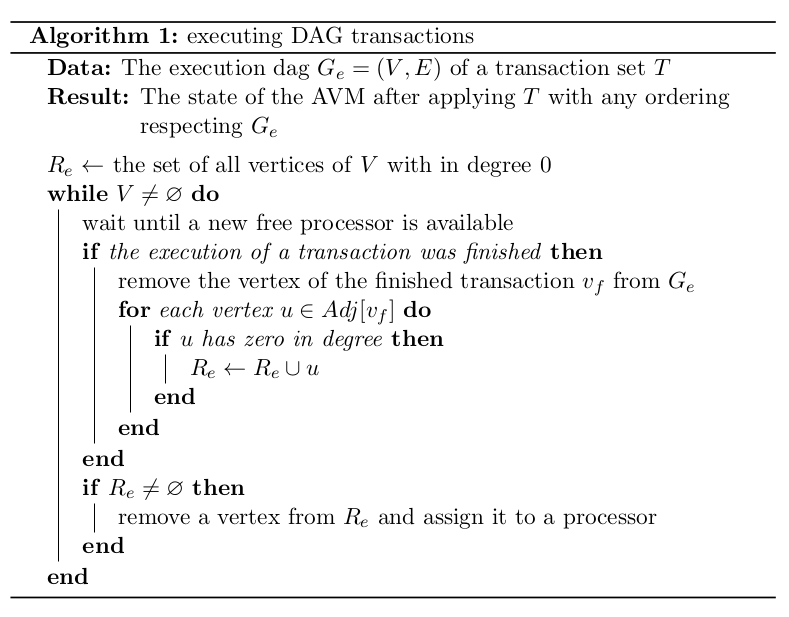
\includegraphics[width=17cm]{../img/Alg1s.png}
\begin{algorithm}
    \DontPrintSemicolon
    \SetKwData{Ready}{$R_e$}\SetKwData{V}{$v_f$}\SetKwData{Graph}{$G_e$}\SetKwData{Vertices}{$V$}\SetKwData
    {Txns}{$T$}
    \KwData{The execution dag $\Graph = (\Vertices,E)$ of transaction set \Txns}
    \KwResult{The state of the AVM after applying \Txns with any ordering respecting \Graph}
    \BlankLine
    \Ready $\gets$ the set of all vertices of \Vertices with in degree 0\;
    \While{$\Vertices \neq \varnothing$}
    {
        wait until a new free processor is available\;
        \If{the execution of a transaction was finished}
        {
            remove the vertex of the finished transaction \V from \Graph\;
            \For{each vertex $u \in Adj[\V]$}
            {
                \If{$u$ has zero in degree}
                {
                    $\Ready \gets \Ready \cup u$\;
                }
            }
        }
        \If{$\Ready \neq \varnothing$}
        {
            remove a vertex from \Ready and assign it to a processor\;
        }
    }
    \caption{executing DAG transactions}\label{alg:exec_dag}
\end{algorithm}

By replacing every undirected edge of a memory dependency graph with a directed edge in such a way that the
resulted graph has no cycles, we will obtain a valid execution DAG. Thus, from a memory dependency graph different
execution DAGs can be constructed with different levels of parallelization ability.

If we assume that we have unlimited number of processors and all transactions take equal time for executing, it
can be shown that by providing a minimal graph coloring to Algorithm~\ref{alg:gen_dag} as input, the resulted
DAG will be optimal, in the sense that it results in the minimum overall execution time.

%##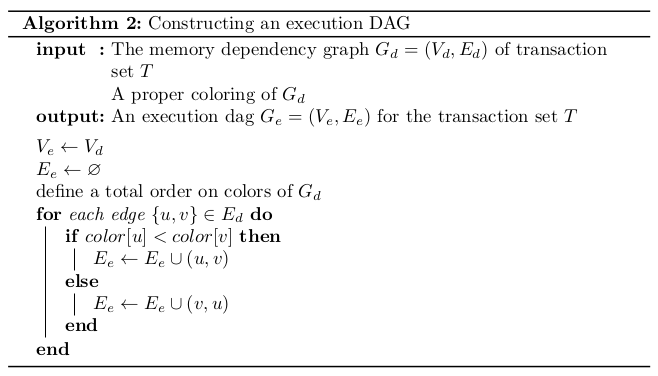
\includegraphics[width=17cm]{../img/Alg2s.png}
\begin{algorithm}
    \DontPrintSemicolon
    \SetKwData{Txns}{$T$}\SetKwData{Gd}{$G_d=(V_d,E_d)$}
    \SetKwInOut{Input}{input}\SetKwInOut{Output}{output}
    \Input{The memory dependency graph \Gd of transaction set \Txns\\A proper coloring of $G_d$}
    \Output{An execution dag $G_e=(V_e,E_e)$ for the transaction set \Txns}
    \BlankLine
    $V_e \gets V_d$\;
    $E_e \gets \varnothing$\;
    define a total order on colors of $G_d$\;
    \For{each edge $\{u,v\} \in E_d$}
    {
        \eIf{$color[u] < color[v]$}
        {
            $E_e \gets E_e \cup (u,v)$\;
        }{
            $E_e \gets E_e \cup (v,u)$\;
        }
    }
    \caption{Constructing an execution DAG}\label{alg:gen_dag}
\end{algorithm}

The block proposer is responsible for proposing an efficient execution DAG alongside his proposed block. This
execution DAG will determine the ordering of block transactions and help validators to validate transactions in
parallel. Since with better parallelization a block can contain more transactions, a proposer is incentivized enough
to find a good execution DAG for transactions.

\subsection{Memory Spooling}\label{subsec:spooling}

When two transactions are dependant and they are connected with an edge \((u,v)\) in the execution DAG,
the transaction \(u\) needs to be run before the transaction \(v\). However, if \(v\) does not read any
memory locations that \(u\) modifies, we can run \(u\) and \(v\) in parallel. We just need to make sure
\(u\) does not see any changes \(v\) is making in AVM memory. This can be done by appropriate versioning
of the memory locations which is shared between \(u\) and \(v\). We call this method \emph{memory spooling}.
After enabling memory spooling between two transactions the edge connecting them can be safely removed from the
execution DAG\@.

\subsection{Concurrent Counters}\label{subsec:concurrent-counters}

We know that in Argennon every transaction needs to transfer its proposed fee to the \texttt{feeSink} accounts
first. This essentially makes every transaction a reader and a writer of the memory locations which store the
balance record of the \texttt{feeSink} accounts. As a result, all transactions in Argennon will be dependant and
parallelism will be completely impossible. Actually, any account that is highly active, for example the account
of an exchange or a payment processor, could become a concurrency bottleneck in our system which makes all
transactions interacting with them dependant.

This problem can be easily solved by using a concurrent counter for storing the balance record of this type of
accounts. A concurrent counter is a data structure which improves concurrency by using multiple memory locations for
storing a single counter. The value of the concurrent counter is equal to the sum of its sub counters and it can
be incremented or decremented by incrementing/decrementing any of the sub counters. This way, a concurrent
counter trades concurrency with memory usage.

Algorithm~\ref{alg:CC} implements a concurrent counter which returns an error when the value of the counter
becomes negative.

%##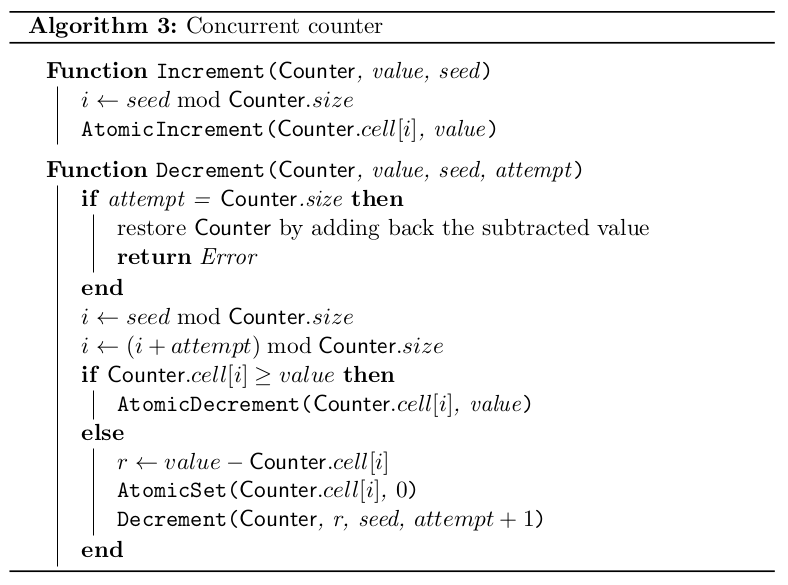
\includegraphics[width=17cm]{../img/Alg3s.png}
\begin{algorithm}
    \DontPrintSemicolon
    \SetKwData{CC}{Counter}
    \SetKwFunction{Inc}{Increment}\SetKwFunction{Dec}{Decrement}\SetKwFunction{AtomInc}{AtomicIncrement}
    \SetKwFunction{AtomDec}{AtomicDecrement}\SetKwFunction{AtomSet}{AtomicSet}\SetKwFunction{Get}{GetValue}
    \SetKwFunction{Acquire}{Lock.Acquire}\SetKwFunction{Release}{Lock.Release}
    \SetKwProg{Fn}{Function}{}{}
    \Fn{\Get{\CC}}
    {
        $s \gets 0$\;
    \Acquire{}\;
    \For{$i \gets 0$ \KwTo $\CC.size - 1$}
    {
        $s \gets s + \CC.cell[i]$\;
    }
    \Release{}\;
    \KwRet{s}\;
    }
    \BlankLine
    \Fn{\Inc{\CC, value, seed}}
    {
        $i \gets seed \bmod \CC.size$\;
    \AtomInc{$\CC.cell[i]$, value}\;
    }
    \BlankLine
    \Fn{\Dec{\CC, value, seed, attempt}}
    {
        \If {attempt = \CC.size}
        {
            restore \CC by adding back the subtracted value\;
            \KwRet{Error}\;
        }
        $i \gets seed \bmod \CC.size$\;
        $i \gets (i + attempt) \bmod \CC.size$\;
    \eIf {$\CC.cell[i] \geq value$}
    {
        \AtomDec{$\CC.cell[i]$, value}\;
    }{
        $r \gets value - \CC.cell[i]$\;
        \AtomSet{$\CC.cell[i]$, $0$}\;
        \Dec{\CC, r, seed, $attempt + 1$}\;
    }
    }
    \caption{Concurrent counter}\label{alg:CC}
\end{algorithm}

It should be noted that in a blockchain application we don't have concurrent threads and therefore we don't need
atomic functions. For usage in a smart contract, the atomic functions of this pseudocode can be implemented like
normal functions.

Concurrent counter data structure is a part of the AVM standard library, and any smart contract can use this data
structure for storing the balance record of highly active accounts.

\subsection{Memory Chunks}\label{subsec:memory-chunks}

In order to further increase the concurrency level of Argennon, we can divide the AVM memory into \emph{chunks}.
Each memory chunk can be persisted using a different ZK-EDB, hence having its own commitment. Then, the
consensus on new values of the commitment of any chunk can be achieved by a different voting committee.

If a transaction does not modify a memory chunk and in the transaction ordering of the block it comes after
any transaction which modifies that chunk, then the execution of that transaction is not needed for calculating
the new commitment of the chunk. Consequently, the voting committee of that memory chunk can safely ignore such a
transaction. The execution DAG of transactions can be used for finding and pruning these transactions as
we see in Algorithm~\ref{alg:prune_dag}.

%##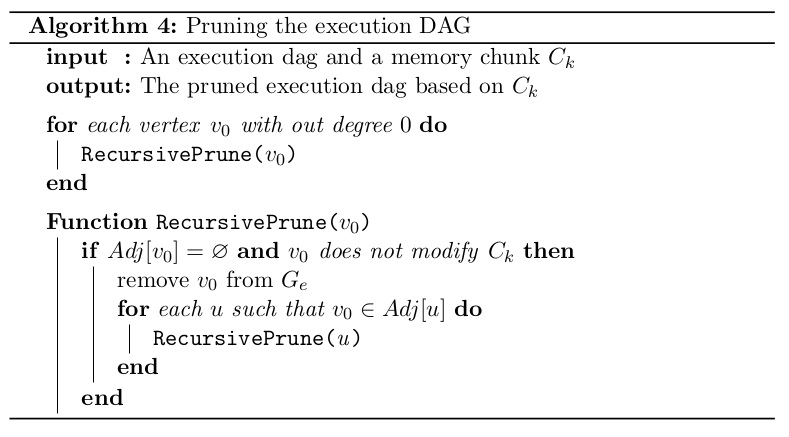
\includegraphics[width=17cm]{../img/Alg4s.png}
\begin{algorithm}
    \DontPrintSemicolon
    \SetKwData{V}{$v_0$}\SetKwData{Graph}{$G_e$}\SetKwData{Chunk}{$C_k$}\SetKwData{Txns}{$T$}
    \SetKwFunction{RPrune}{RecursivePrune}
    \SetKwProg{Fn}{Function}{}{}
    \SetKwInOut{Input}{input}\SetKwInOut{Output}{output}
    \Input{An execution dag \Graph and a memory chunk \Chunk}
    \Output{The pruned execution dag based on \Chunk}
    \BlankLine
    \For{each vertex \V with out degree $0$}
    {
        \RPrune{\V}\;
    }
    \BlankLine
    \Fn{\RPrune{\V}}
    {
        \If{$Adj[\V] = \varnothing$ {\bf and} \V does not modify \Chunk}
        {
            remove \V from \Graph\;
            \For{each $u$ such that edge $(u,\V)$ was in \Graph}
            {
                \RPrune{u}\;
            }
        }
    }
    \caption{Pruning an execution DAG}\label{alg:prune_dag}
\end{algorithm}

If we choose chunks in a way that most transactions only modify memory locations of one chunk,
likely many transactions of a block only need to be validated by one voting committee and can be validated in
parallel by different committees.

Because the voting committees are selected by random sampling, by choosing large enough samples we can make sure
that having multiple voting committees will not change the security properties of the Argennon agreement protocol.